\documentclass{report}
\usepackage{amsmath, amssymb}
\usepackage{acronym}
\usepackage{graphicx}
\usepackage{placeins} 
\usepackage{tikz}

\acrodef{ML}[ML]{machine learning}
\acrodef{BERT}[BERT]{bidirectional encoder representations from transformers}
\acrodef{KL}[KL]{Kullback-Leibler}
\acrodef{FLOPs}[FLOPs]{floating point operations}

\begin{document}

\title{BERT Hangman Project}
\author{Bernardo Camajori Tedeschini}
\date{4 August 2024}

\maketitle

\section*{Challenge description}
The idea of the challenge is to implement a novel strategy that uses a \ac{ML}
model to infer the next letter prediction in the Hangman game. 
The model has to be trained on a dataset of words \textit{words\_250000\_train.txt} and must achieve an accuracy higher than
55\% on a single test game. 

Now, the first questions was: what should be roughly the test accuracy on the single letter prediction to achieve an accuracy of 
55\% on a single test game? We know that we have at disposal only 6 attempts to guess the word, so to win the game 
we need to guess the word in less than 6 attempts. 
Given the maximum number of unique letters in a word (15 in the worst case), we define:
\begin{itemize}
    \item $p$ as the probability of guessing a single letter,
    \item $X_n$ as the number of wrongly guessed letters in a word with $n$ unique letters. \\ ${X_n \sim \text{Bin}(n, 1-p)}$.
\end{itemize}
Therefore, we have a worst case scenario where the probability of winning the game is given by:
\begin{equation}
    W(p) = P(\text{win} | p) = P(X_{15} \le 5)= \sum_{i=0}^{5} P(X_{15} = i) = \sum_{i=0}^{5} \binom{15}{i} (1-p)^i (p)^{15-i}.
\end{equation}
By plotting the probability of winning the game as a function of the probability 
of guessing a single letter, i.e., $W(p)$, we obtain the following plot:
\begin{figure}[!h]
    \centering
    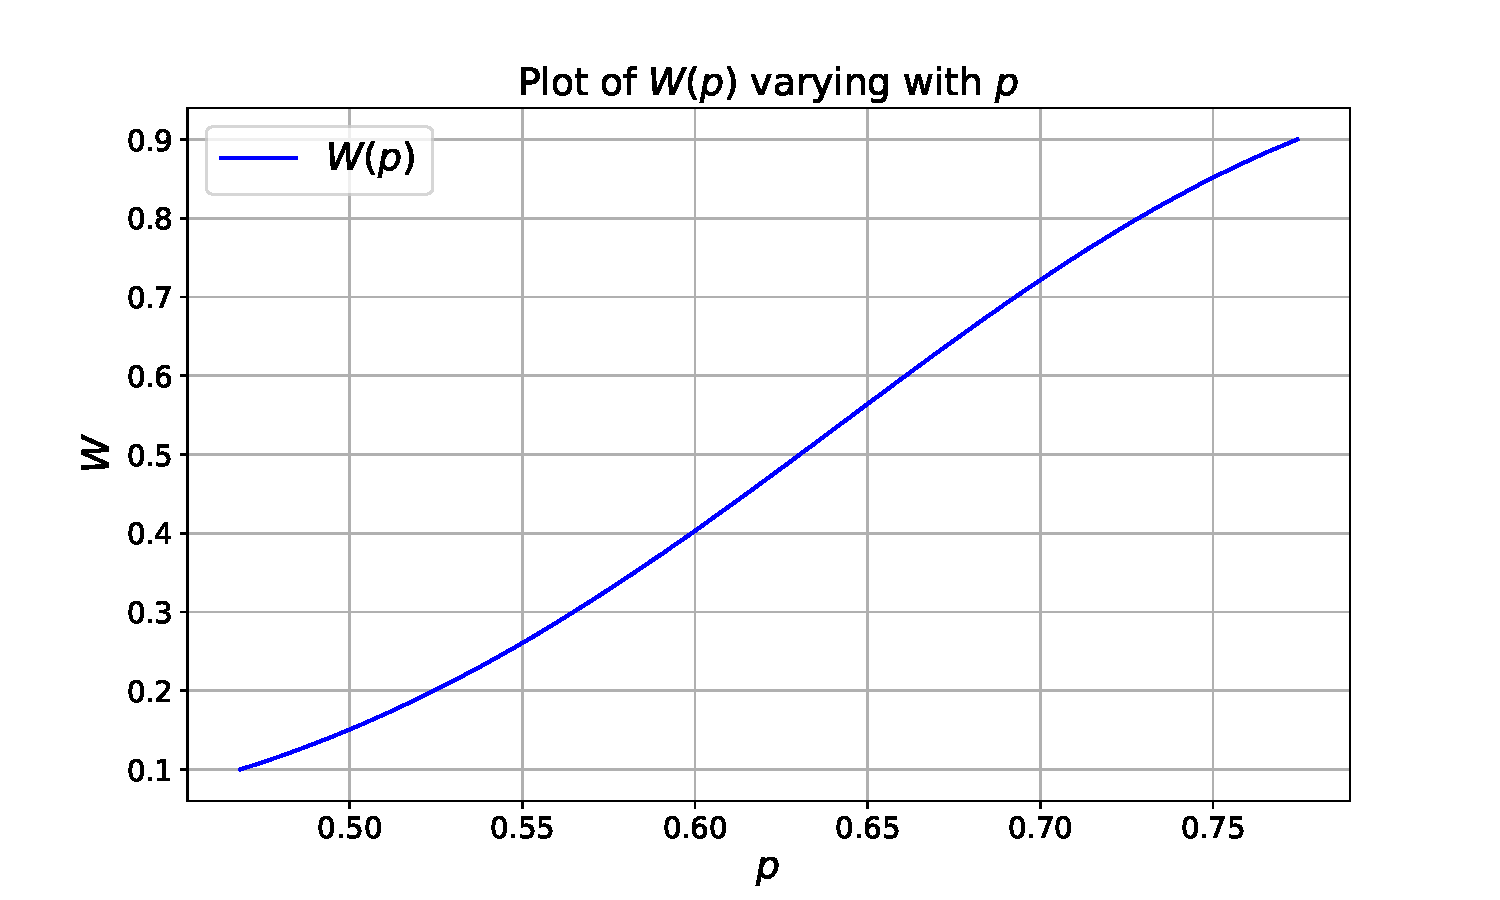
\includegraphics[width=0.7\textwidth]{figures/Figure_1.pdf}
    \caption{Probability of winning the game as a function of the probability of guessing a single letter.}
\end{figure}

We note that the probability of correct letter prediction $p$ must be 
higher than 0.65 to achieve a probability of winning the game higher than 0.55. 


\section*{Model Composition}
Given the peculiarities of the Hangman game, i.e., prediction of masked tokens (letters), we can define the 
problem as a conventional mask language model task. 
One of the most popular models for this task in language processing is the 
\ac{BERT} model. \ac{BERT} takes inspiration from the encoder part of the transformer model to 
produce embeddings for the input tokens which contain contextual, as well as positional information of the tokens.
The model composition is based on the following components:
\begin{itemize}
    \item A tokenizer that maps the input letters to a sequence of tokens. The vocabulary size is $V$ (26 characters + 2 special tokens, i.e., '$\$$' for the unknown token and '\_' for the padding token).
    Output size: $B \times T$, where $B$ is the batch size and $T$ is the maximum token length.
    \item A token embedding layer, which maps the input tokens to their corresponding embeddings. Output size: $B \times T \times E$, where $E$ is the embedding size.
    \item A positional embedding layer, which maps the position of the tokens to their corresponding embeddings, since the transformer model does not have a built-in positional information. Output size: $B \times T \times E$.
    \item A stack of transformer encoders, which process the input embeddings to produce contextual embeddings. 
    Each encoder is composed of a multi-head self-attention mechanism and a feed-forward neural network with $F$ hidden units. Moreover, each encoder has also residual connections and layer normalization modules. Output size: $B \times T \times E$.
    \item A generator layer, which maps the contextual embeddings to the output. An important note here is that the model will not perform multi-classification for each token, 
    since in the Hangman game we are only interested in the prediction of the correct letter in the masked tokens. 
    Therefore, we can effectively produce an output of size $B \times V$ that predicts the distribution of the letters in the masked tokens.
\end{itemize}
Regarding computational resources, the model has a total of $L=4$ layers, $H=4$ heads, $E=256$ embedding size, and $F=1024$ hidden units.
The total number of \ac{FLOPs} is given by: $6.9 \cdot 10^9$ (precisely 6,927,371,392). 


\section*{Dataset Generation}
For the dataset generation, we need to create a dataset that is compatible with the \ac{BERT} model.
In particular, we need to create couples of input-output pairs, where the input is a sequence of tokens (un/masked tokens)
and the output is the distribution of the letters in the masked tokens.
Moreover, in the game of Hangman, we also have as input the wrongly guessed letters, 
which can be exploited by the model to improve the prediction of the masked tokens.
To sum up, the input-output pairs are defined as follows:
\begin{itemize}
    \item Input1: a sequence of tokens of $B \times T$, where the masked tokens are replaced by the special token '$\$$'. 
    The masked amount is chosen uniformly at random for each word in the dataset in the range [1, ${num\_unique\_letters - 1}$]. 
    This is done to simulate different levels of difficulty in the game.
    \item Input2: the boolean wrongly guessed letters of size $B \times V$, whose number is chosen with a truncated Exponential distribution with $\lambda = 1$ (see Fig. \ref{fig:fig2}).
    I chose this distribution since the most common and difficult case is the beginning of the game, where the number of wrongly guessed letters is low.
    When, the number of wrongly guessed letters is high, the game is almost solved and the model can easily predict the masked tokens without the need of the wrongly guessed letters.
    \item Input3: the boolean source mask for the masked-self-attention mechanism of size $B \times T$, which is used to avoid the model focusing on the masked tokens.
    \item Output: the distribution of the letters in the masked tokens of size $B \times V$.
\end{itemize}

\begin{figure}[!h]
    \centering
    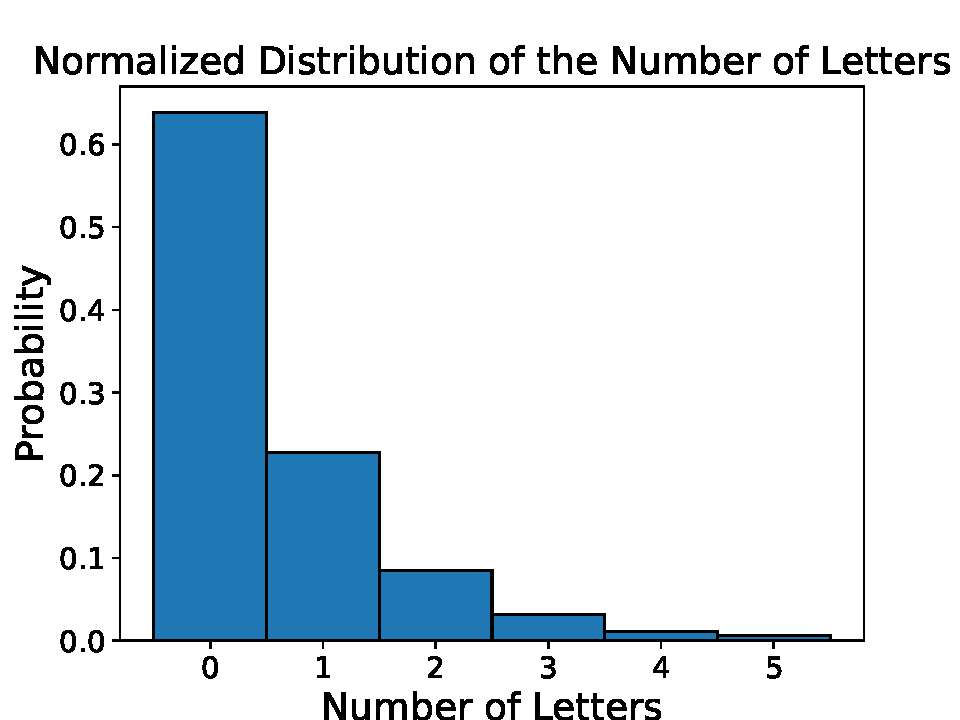
\includegraphics[width=0.6\textwidth]{figures/Figure_2.pdf}
    \caption{Truncated Exponential distribution with $\lambda = 1$.}
    \label{fig:fig2}
\end{figure}


\section*{Loss Function}
The final predicted distribution is obtained from the model output by applying a
generator-mask which sets to zero the probability of the letters that are not in the masked tokens or that are wrongly guessed.
In this way the model cannot predict the already visible letters or the wrongly guessed letters.
After a softmax function, the predicted distribution is compared with the true distribution of the letters in the masked tokens using
the \ac{KL} divergence loss function:
\begin{equation}
    \text{Loss} = \sum_{i=1}^{V} p_i \log \left( \frac{p_i}{q_i} \right),
\end{equation}
where $p_i$ and $q_i$ are the true and predicted normalized frequencies of the $i$-th token, respectively.
As regarding the accuracy, I defined it as:
\begin{equation}
    \text{Accuracy} = \frac{\sum_{i=1}^{N} \mathbf{1}(\hat{y}_i \in y_i)}{N},
\end{equation}
where:
\begin{itemize}
    \item $N$ is the total number of words in the dataset,
    \item $\hat{y}_i$ is the model's predicted letter for the $i$-th word,
    \item $y_i$ is the set of possible correct letters for the $i$-th word,
    \item $\mathbf{1}(\hat{y}_i \in y_i)$ is the indicator function that returns 1 if the predicted letter $\hat{y}_i$ is within the set of correct letters $y_i$, and 0 otherwise.
\end{itemize}

\section*{Training and Validation Results}
For the validation dataset, I adopted a disjoint set of 74,000 words created by 
subtracting from online words dataset the words used for the training dataset.
In Fig. \ref{fig:fig3} we can see the training and validation dataset in terms of number of unique letters and word length.

\begin{figure}[!h]
    \centering
    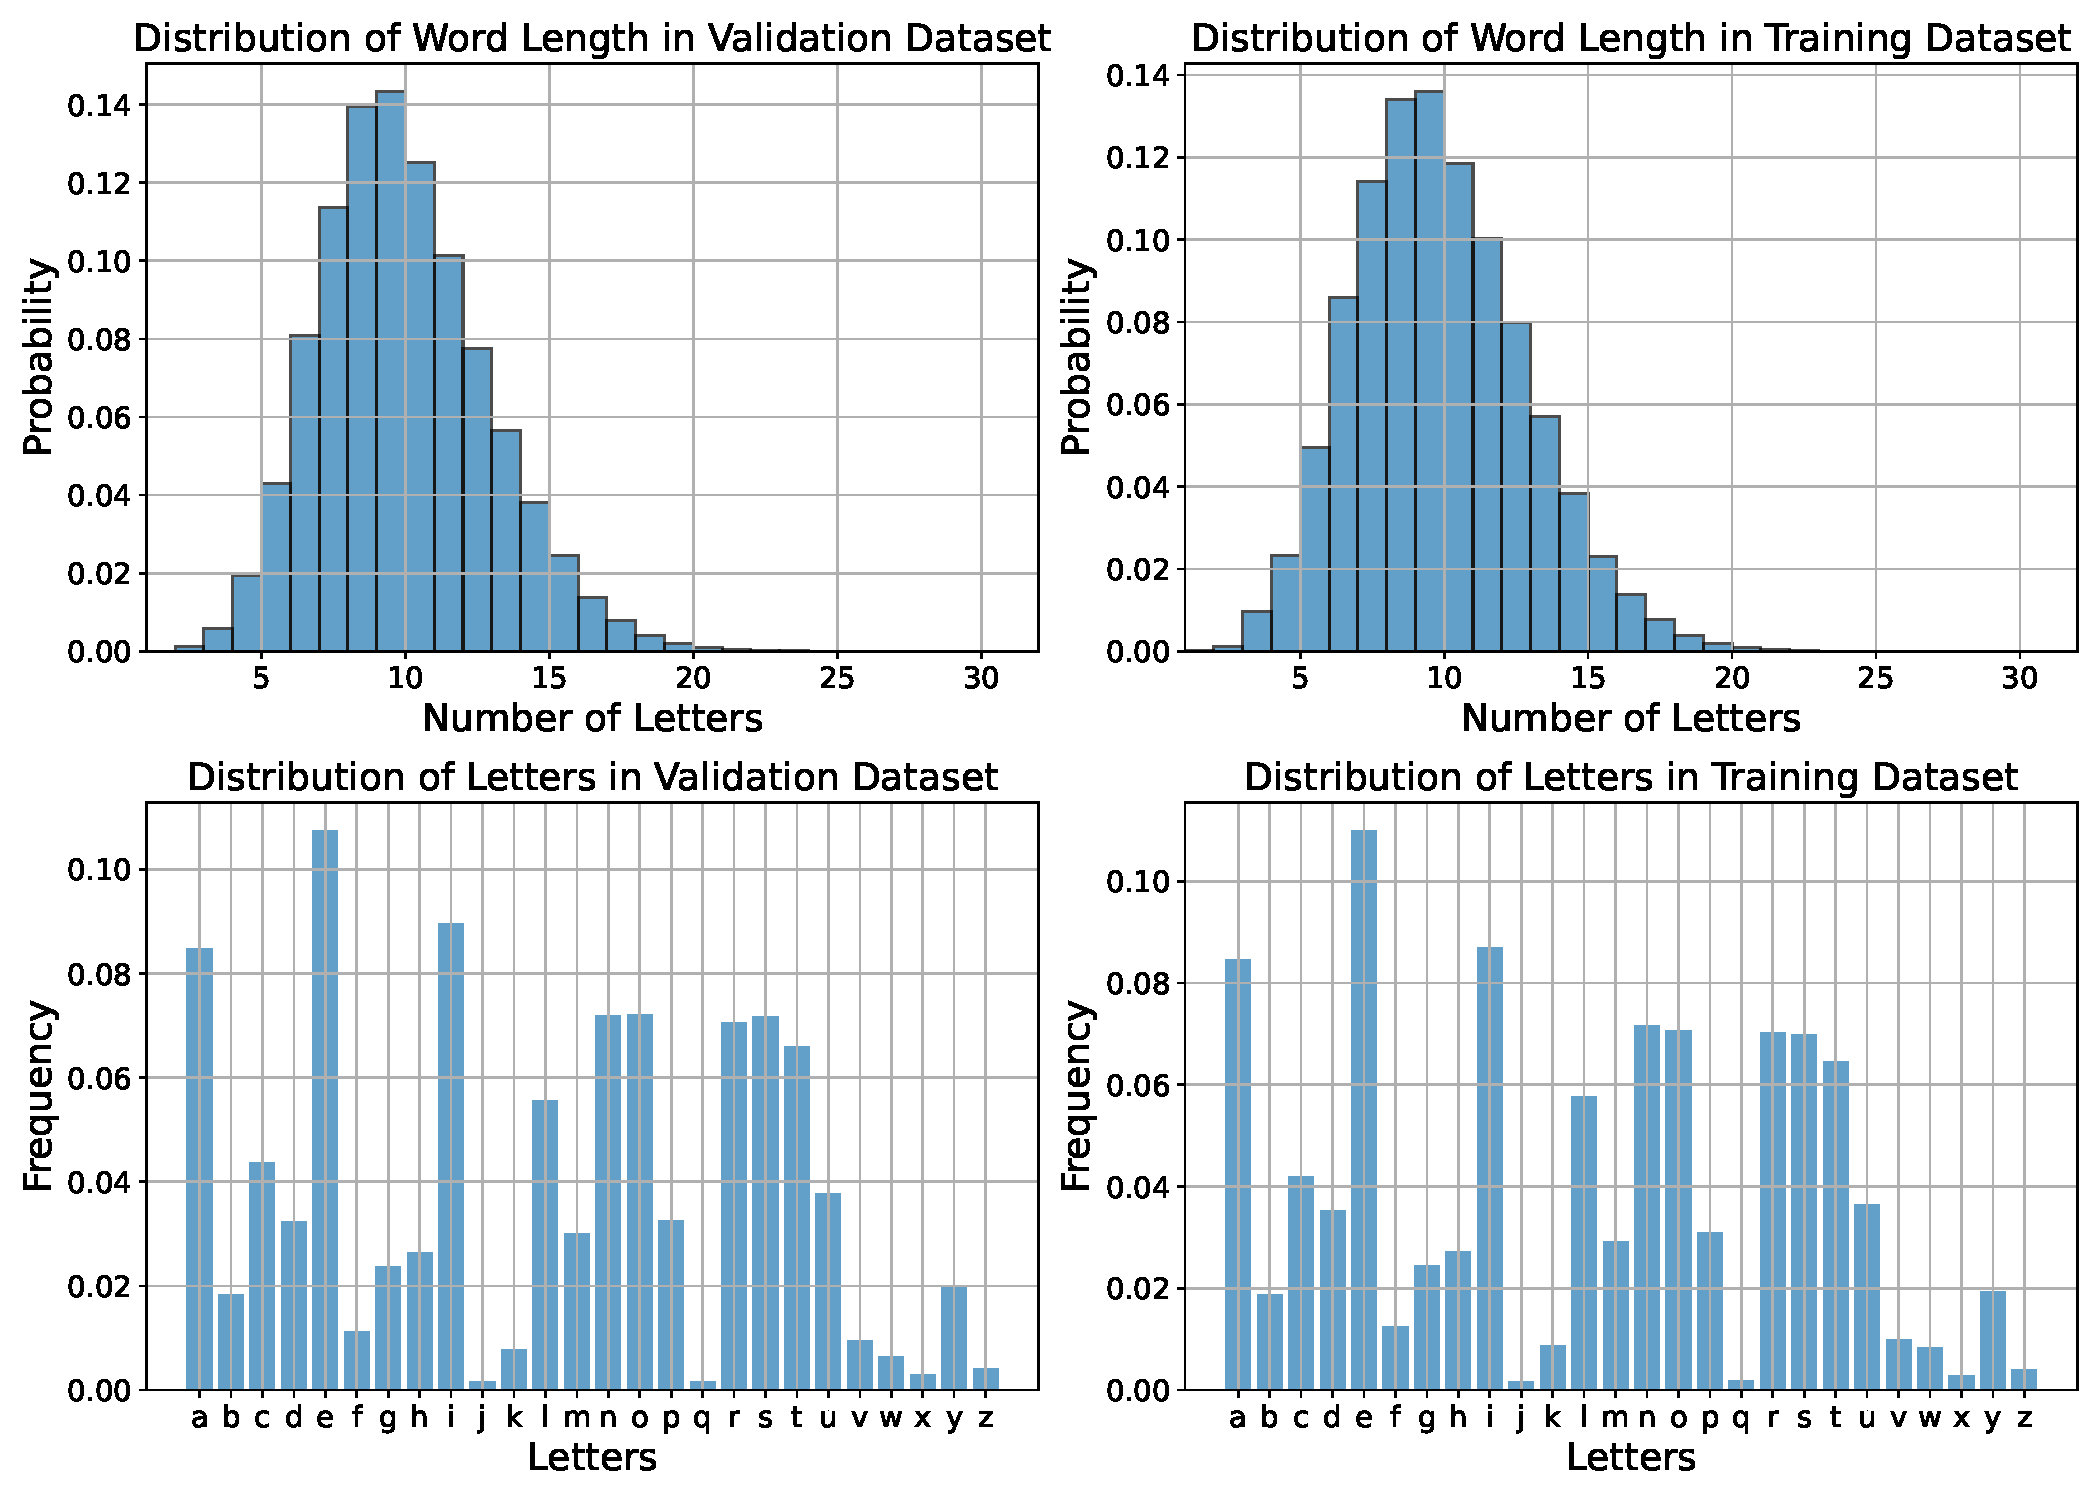
\includegraphics[width=1\textwidth]{figures/Figure_3.pdf}
    \caption{Training and validation dataset in terms of number of unique letters and word length.}
    \label{fig:fig3}    
\end{figure}

I now report in Fig. \ref{fig:fig4} the training loss and validation accuracy as a function 
of the number of seen words (i.e., about about 400 epochs with a batch size of 512 words). 
To avoid overfitting, as well as to obtain a reliable performance on the validation set, both the datasets where 
recomputed at each epoch to have different masks and wrongly guessed letters.
From the figure, we can observe that the achieved accuracy on the validation set is about 0.68, 
which is higher than the required 0.65. 
Indeed, by testing the model in a local simulated game, we obtain a success rate of 0.58 in 7000 tries.

% Tikz for the training loss and validation accuracy ()
\begin{figure}[!h]
    \centering
    \begin{tikzpicture}
        \node at (-3,0) {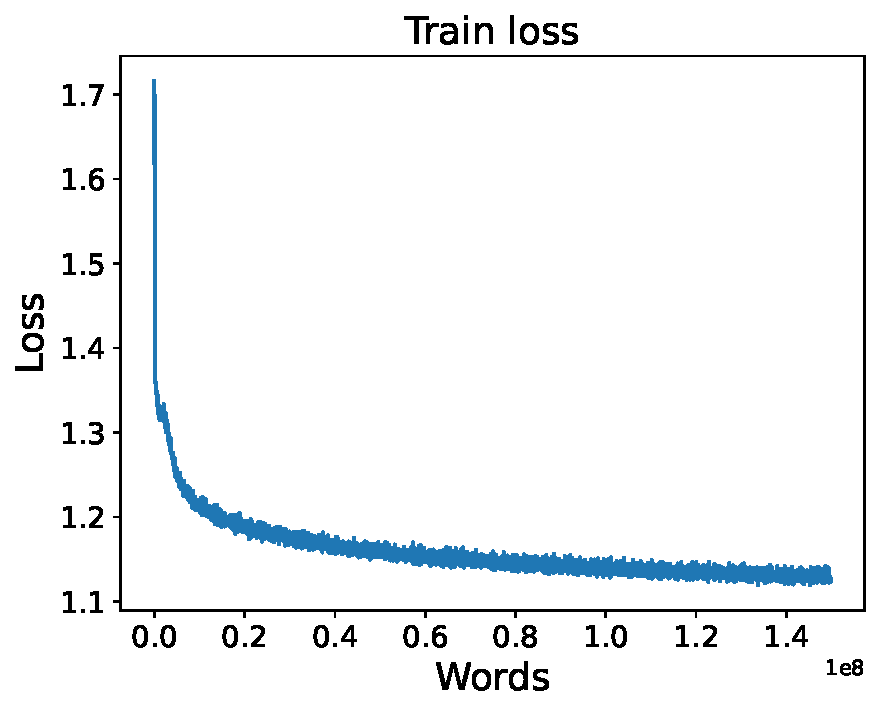
\includegraphics[width=0.5\textwidth]{figures/Figure_4_loss.pdf}};
        % \node at (-3,-2.5) {Training Loss};
        \node at (3,0) {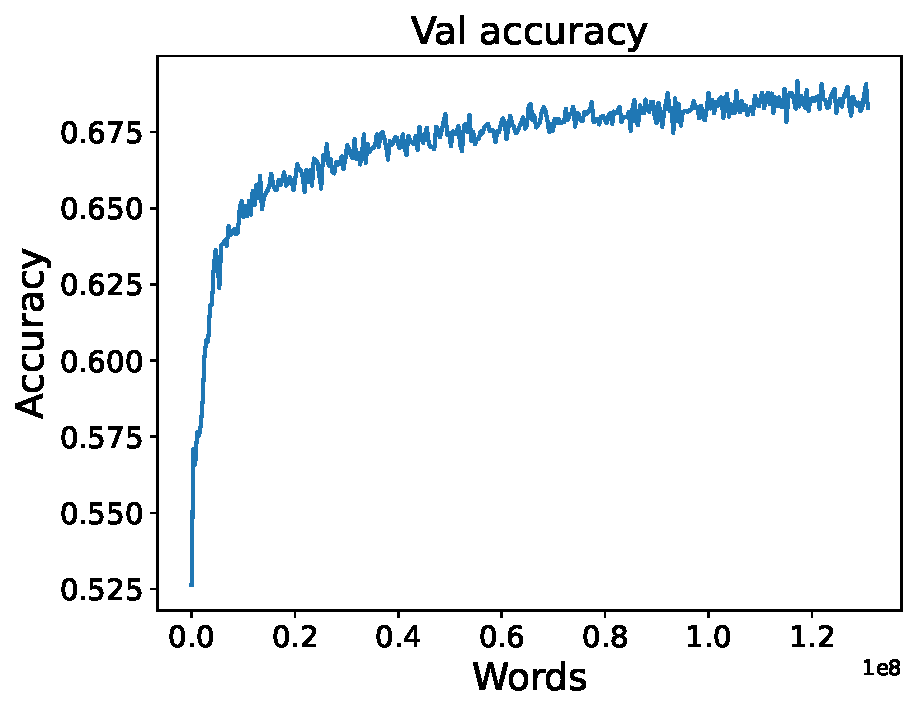
\includegraphics[width=0.5\textwidth]{figures/Figure_4_acc.pdf}};
        % \node at (3,-2.5) {Validation Accuracy};
    \end{tikzpicture}
    \caption{Training loss and validation accuracy as a function of the number of seen words.}
    \label{fig:fig4}
\end{figure}


\section*{Conclusion}
In this report, I presented a novel strategy to solve the Hangman game using a \ac{BERT} model.
The model is trained on a dataset of 250,000 words and achieves 
a game-accuracy of about 0.58, which outperforms the default strategy (0.18).
Possible future improvements could be the integration of a reinforcement learning algorithm to
optimize the wrongly guessed letters, as well as the masked tokens.

\section*{Data and Code}
The data is available in the folder \texttt{DB}, comprising the training and validation datasets.
The main code files are as follows:
\begin{itemize}
    \item \texttt{main.py}: to train and test the model. 
    The saved model is available in the folder \texttt{Classes/model/Saved\_models}, 
    whereas the training and validation logs are available in the folder \texttt{Classes/model/Output\_results}.
    \item \texttt{hangman\_local\_user.py}: to test the model in a local simulated game using the validation dataset.
    \item \texttt{hangman\_api\_user.ipynb}: to test the model in a real game using the API.
    \item folder \texttt{Classes}: containing the main classes for the solver, model, dataset, and optimizer.
\end{itemize}


\end{document}